\documentclass{article}
\usepackage[utf8]{inputenc}
\usepackage[margin =1in,includefoot]{geometry}
\usepackage{indentfirst}
\usepackage{graphicx}
\usepackage{caption}
\usepackage{tikz}
\usetikzlibrary{shapes, arrows, calc, arrows.meta, fit, trees,positioning}
\usepackage{float}
\usepackage{amsmath,mathtools}
\usepackage{listings}
\usepackage{xcolor}

\definecolor{backcolour}{rgb}{0.95,0.95,0.92}

\lstdefinestyle{mystyle}{
    backgroundcolor=\color{backcolour},
    numberstyle=\small,
    numbers=left,  
}

\title{COL351 Assignment 1}
\author{Aniket Gupta \hspace{2cm}  Aayush Goyal \\
    2019CS10327 \hspace{2.3cm} 2019CS10452}
\date{September 2021}

\lstset{style=mystyle}

\begin{document}

\maketitle

\section{Minimum Spanning Tree}
\subsection{}

Let T be the MST generated by Kruskal algorithm with edges $e_{1}<e_2<e_3<...e_{n-2}<e_{n-1}$ and let T' be any other MST of G with edges $\Bar{e}_1<\Bar{e_2}<\Bar{e_3}<...\Bar{e_{n-2}}<\Bar{e_{n-1}}$.
\\
We need to prove that $e_i$ and $\Bar{e_i}$ are the same edge in G ($\forall$ $1<=i<n$). We prove this by induction.\\
\textbf{Induction Predicate}:
\\
H(i) ::= $e_j$ and $\Bar{e_j}$ are the same edge in G $\forall$ $1<=j<=i$
\\
where $1<=i<n$
\\
\textbf{Base Case} - Proof that $e_1$ and $\Bar{e_1}$ are the same edge in G.
\\
We prove this by contradiction.
\\
Let us assume that ${e_1}$ does not lie in T'. Adding ${e_1}$ to T' to give a cycle C in T'. Note that all the edges in C will have weight greater than weight of ${e_1}$ since it is the edge with smallest weight in G. Now removing any edge, except ${e_1}$, from C will give another tree with smaller total weight than that of T'. This contradicts the fact that T' is a MST.\\
Thus, ${e_1}$ must lie in T'.
\\
\textbf{Induction Step}:
\\
Assume H(i) is true for some $1<=i<n-1$.\\
We need to show H(i) $=>$ H(i+1).
\\
\textbf{Claim 1}: $e_{i+1}$ in T and $\Bar{e_{i+1}}$ in T' are the same edge in G.\\
\textbf{Proof of claim 1}:
We prove this by contradiction. Let us assume that $e_{i+1}$ and $\Bar{e_{i+1}}$ are different edges in G. Adding $e_{i+1}$ in T' will give a cycle C in T'. Now, all the edges in C, except $e_{i+1}$, cannot belong to {$e_1$, $e_2$, ..., $e_i$} since these edges are also in T due to induction hypothesis and thus cannot form a cycle with $e_{i+1}$ (since T is a tree). Thus, atleast one edge in C must be in {$\Bar{e_{i+1}}$, $\Bar{e_{i+2}}$, ... , $\Bar{e_{n-1}}$}. Let that edge be e'. \\
Observations:
\\{$e_1$, $e_2$, ..., $e_i$, $e_{i+1}$} is acyclic (since these edges are in T) 
\\{$e_1$, $e_2$, ..., $e_i$, $\Bar{e_{i+1}}$} is acyclic (since these edges are in T')
\\ From the above two observations and the fact that edges are traversed in increasing order of weight in Kruskal algorithm, we conclude that weight($\Bar{e_{i+1}}$) $>=$ weight($e_{i+1}$).
\\But, we assumed that $\Bar{e_{i+1}}$ and $e_{i+1}$ are different, thus weight($\Bar{e_{i+1}}$) $>$ weight($e_{i+1}$).
This implies that weight(e') $>$ weight($e_{i+1}$). Thus removing e' from C will give a tree with total weight smaller than that of T'. This contradicts the fact that T' is a MST. Thus, $e_{i+1}$ and $\Bar{e_{i+1}}$ are same edge in G.
\\
\\
By claim 1 and the induction hypothesis H(i), we get that H(i+1) is true.
\\
Thus by induction, we showed that T' and T have the same edges. Note that T' was any arbitrarily possible MST of G and thus this is true for all the MSTs of G. This implies that G has a unique MST.

\subsection{}
Approach: The basic approach we have used is to detect cycles in the graph G and remove edge with maximum weight in the cycles found. We have used DFS to detect cycles in the graph. In each DFS traversal, one edge from G, which also belongs to any cycle in G, is removed.
\\
\\
\textbf{Claim 1}: For any cycle C in G, the edge with maximum weight in the cycle C cannot belong to a MST.
\\
\textbf{Proof of claim 1}:
\\
We prove this claim by contradiction. Let us assume that e' = (u,v) be the edge with maximum weight in cycle C and it lies in a MST T. Removing e' breaks T in two subtrees T1 and T2. Note that T1 and T2 both contain one end of e' (because they can't be in the same tree, because that would mean they are connected even after the removing the edge connecting them and we know they were initially a part of a tree T and there exists only one unique path in a tree). Now, the other edges of C (except e') connects u and v in G. Thus, there must be atleast one edge in C (except e') with its end-points in different subtrees. Let that edge be $\Bar{e}$. Note that weight($\Bar{e}$) $<$ weight(e'), since e' was the maximum weight edge in C and all the edges in G have distinct edge weight. Join T1 and T2 with $\Bar{e}$ gives another tree with total weight less than that of T. But, it is not possible since T is a MST of G. Thus, by contradiction, for any cycle C in G, the edge with maximum weight in the cycle C cannot belong to a MST.
\\

\textbf{Algorithm:}
\lstinputlisting[firstline =1]{1b.txt}
In the above algorithm, get\_MST() is main function that is called to get MST for a graph G with distinct edge weights. dfs(node) and refresh\_nodes() are helping methods in the algorithm. In for loop (line 54-56) of get\_MST() method, we are calling dfs(1) method with 1 as the root after refreshing all the nodes (marking all nodes as unvisited, setting parent and tree edges to default value -1).\\
The dfs(node) method performs normal dfs along with detecting a cycle and removing edge with maximum weight from that cycle (line 40-50).
\\
\\
\textbf{Proof for Correctness of the above algorithm:}

\begin{enumerate}
\item By claim 1, we can say that if we find an edge e that belongs to any cycle C in G such that e is the maximum weight edge in C, then we can remove e from G to get graph G' such that MST of G and G' will be same.
\item After removing an edge from a cycle C in a connected graph G, the new graph will still be connected.
\item A connected graph with more than n-1 edges must have a cycle. And a connected graph with n-1 edges cannot have a cycle.
\end{enumerate}

From the above three points, we can see that after each iteration of the for loop (line 54-56), we get a new tree with one less edge than the previous tree such that the MSTs of both the trees are exactly the same. Also, this loop runs for (m-n+1) times and thus we are left with a connected graph with n-1 edges (i.e. a tree) with same MST as the original tree. This proves the correctness of the algorithm.
\\\\
\textbf{Time Complexity Analysis:}
\\Making a DFS traversal and removing an edge from a cycle can be done in O(n+m) time complexity. In our case, $m<=n+8$ and thus time complexity of single DFS traversal is O(n). Also, DFS traversal (and thus edge removal from a cycle) is made for maximum 9 times, since $m<=n+8$ and a tree has n-1 edges. \textbf{Thus, the total time complexity is} $O(9n) = O(n)$. 

\newpage
\section{Huffman Encoding}
\subsection{}
We will use Huffman Encoding algorithm to solve this problem. We keep replacing two letters with least frequencies (say $f_1$ and $f_2$) with a new auxiliary letter with frequency $f_1+f_2$ until only 1 auxiliary letter is remaining. Then start building the Huffman tree starting with the one auxiliary letter remaining and expand the tree by making its two children, the two letters that were used in the previous step to obtain this auxiliary letter. Keep expanding the tree as long as any auxiliary letter is remaining as a leaf in the tree. This will give the final Huffman tree.
\\
\\
\textbf{Claim 1}: The sum of first i Fibonacci numbers is Fib(i+2)-1.
\\
\textbf{Proof for the claim 1:}
\\
Let us denote sum of first $i$ Fibonacci numbers by $S(i)$. We want to prove that $S(i) = Fib(i+2)-1 \forall i>0$.
\\
\textbf{Base Case: }
\\
S(1) = 1 = 2-1 = Fib(2)-1
\\
\textbf{Induction Step:}
\\
Let this claim be true for some i i.e., S(i) = Fib(i+2)-1. 
\\Now, S(i+1) = S(i)+Fib(i+1) = Fib(i+1)+Fib(i+2)-1 = Fib(i+3)-1. Thus, the claim is also true for i+1. \\Thus, the given claim is true for all values of i ($>$0).
\\\\
\textbf{Claim 2:} In the Huffman tree for the frequency vector as first n Fibonacci numbers, the letter with frequency Fib(n) will be chosen in the last iteration of replacing two letters with smallest frequencies and thus will be at depth 1 in the Huffman tree.
\\
\textbf{Proof for claim 2:}
\\
Note that in the huffman encoding algorithm, we keep choosing two letters with minimum frequencies to replace with an auxiliary letter during the initial step. Also, the sum of all the frequencies always remains constant. These points along with claim 1 implies that letter with frequency Fib(n) (along with an auxiliary letter with frequency Fib(n+1)-1) will be chosen to be replaced with another auxiliary letter only in the last.
\\\\
Thus, from the above two claims, we get that in the Huffman tree for frequency vector as first n Fibonacci numbers, the two children subtrees of the root node will be (1) letter with frequency Fib(n) and (2) Huffman tree for frequency vector as first n-1 Fibonacci numbers.
\\
Thus, recursively building the Huffman tree, we get the following:

\begin{figure}[H]
    \begin{center}
        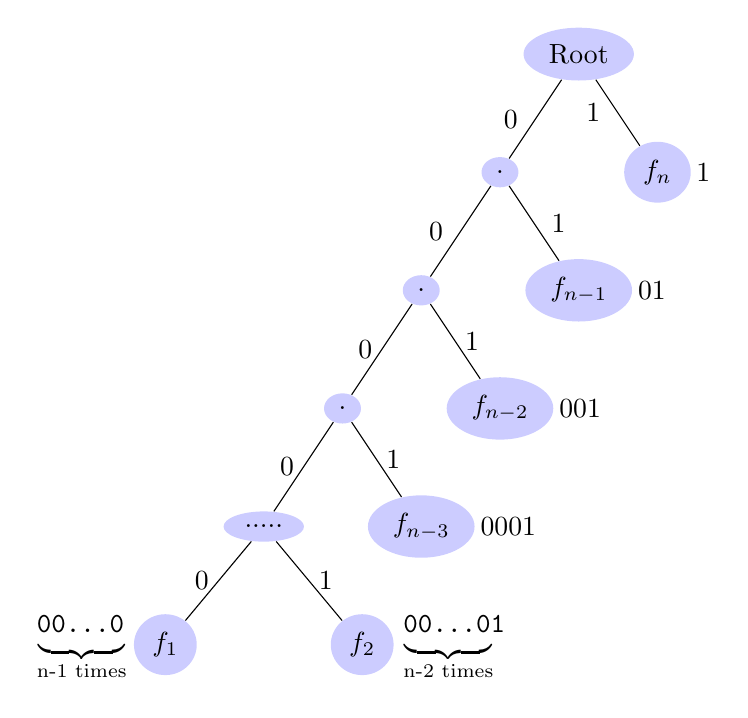
\begin{tikzpicture}[level distance=1.5cm,
            level 1/.style={sibling distance=2cm},
            level 2/.style={sibling distance=2cm},
            level 3/.style={sibling distance=2cm},
            level 4/.style={sibling distance=2cm},
            level 5/.style={sibling distance=2.5cm},
            tree node/.style={ellipse, fill = blue!20},
            every child node/.style={tree node}]
            
            \node[tree node] (Root) {Root}
                child {
                node {.} 
                child { node {.} 
                            child{ 
                                node {.} 
                                child{
                                    node {.....}
                                    child { 
                                    node (f1) {$f_1$} edge from parent node[left] {0}
                                    }
                                    child{node (f2) {$f_2$} edge from parent node[right] {1}
                                    }
                                    edge from parent node[left] {0}
                                }
                                child{ node (fn-3) {$f_{n-3}$} edge from parent node[right] {1}
                                }
                                edge from parent node[left] {0}
                            }
                            child{ node (fn-2) {$f_{n-2}$} edge from parent node[right] {1}
                            }
                            edge from parent node[left  =0.1 cm] {0} 
                        }
                child { node (fn-1) {$f_{n-1}$} 
                            edge from parent node[right = 0.1 cm] {1} }
                    edge from parent node[left = 0.1cm] {0} 
                }
            child {
                node (fn) {$f_n$}
                edge from parent node[left = 0.1cm] {1} 
            };
        \draw (fn) node[right = 0.37 cm,draw=none,fill=none](){$1$};
        \draw (fn-1) node[right = 0.63 cm,draw=none,fill=none](){$01$};
        \draw (fn-2) node[right = 0.63 cm,draw=none,fill=none](){$001$};
        \draw (fn-3) node[right = 0.63 cm,draw=none,fill=none](){$0001$};
        \draw (f1) node[left = 0.4 cm, draw=none,fill=none](){$
\mathrlap{\underbrace{\phantom{\texttt{00...0\strut}}}_{\text{n-1 times}}}\texttt{00...0}%
$};
        \draw (f2) node[right =0.4 cm, draw=none,fill=none](){$ 
\mathrlap{\underbrace{\phantom{\texttt{00...0\strut}}}_{\text{n-2 times}}}\texttt{00...0}%
\texttt{1}%
$};
    
        \end{tikzpicture}
        \caption*{\textbf{Huffman encoding tree for frequency vector as first n Fibonacci numbers}}
    
    \end{center}
\end{figure}

Thus, for frequency vector with first $n$ Fibonacci numbers, optimal binary Huffman encoding for letter with frequency $Fib(i) =\mathrlap{\underbrace{\phantom{\texttt{00...0\strut}}}_{\text{n-i times}}}\texttt{00...0}%
\texttt{1}%
$ for i$>$1(where no. of 0s in start is n-i and they are followed by 1).
\\\\
Huffman encoding for letters with frequency 1 are 
$
\mathrlap{\underbrace{\phantom{\texttt{00...0\strut}}}_{\text{n-1 times}}}\texttt{00...0}%
$
and 
$ 
\mathrlap{\underbrace{\phantom{\texttt{00...0\strut}}}_{\text{n-2 times}}}\texttt{00...0}%
\texttt{1}%
$
\\\\\textbf{Corner case:} For n = 1, character with frequency Fib(1) = 1 can be encoded as 0
\newpage
\subsection{}

Since these are 16 bit characters then there are a total of $2^{16}$ characters that are possible. We will denote $2^{16}$ by $n$. Let the frequencies of them be $f_1, f_2, ... , f_n$ and they are in increasing order. It is given that $f_n < 2f_1$. Let's denote the symbol with $a_1, a_2, ... ,a_n$
\\\\
Now let's say we consider any numbers from them. Let them be $f_i$ and $f_j$. 
\\\\
\textbf{Claim 1:} $f_i+f_j > f_n$ (and hence greater than every other frequency).
\\ 
\textbf{Proof of claim 1:}

$f_i >= f_1$

$f_j >= f_1$\\
Thus $f_i+f_j >= 2f_1$\\ 
Also it is given that $f_n < 2f_1$, thus this directly proves that $f_i+ f_j > f_n$.
\\\\
Now in Huffman encoding we choose the 2 vertices with minimum frequency (say $f_1$ and $f_2$) and combine them. Then place a node with value $f_1+f_2$ and then recursively solve the problem further. The symbols that will be chosen in the next iteration will be $f_3$ and $f_4$, since $f_3<=f_4<= f_5<= f_n < f_1+ f_2$. And hence we will join $f_3$ and $f_4$ from the set and replace with a node of value $f3+f4$. This will go on and ultimately we will end with these frequencies in the set: $(f_1+f_2), (f_3+f_4), (f_5+f_6), ... ,(f_{n-1}+f_n)$, thus all of the initial $a_i's$ will be combined.
\\\\
\textbf{Claim 2:} let $f$ be a set of numbers of size $n$, here $n$ is a power of 2. Let the numbers be $f_1, f_2, f_3, f_4, ... ,f_{n-1}, f_n$. If we make another set $ff$ from it such that ${ff}_i = f_{2i-1} + f_{2i}$, then it is of half the size and also follows the property that maximum element is less than twice the minimum element. 
\\
\textbf{Proof of Claim 2:} The minimum element of $ff$ set is $f_1+f_2$ and the maximum element is $f_{n-1}+f_n$. Now we know that\\ 
$f_n < 2f_1$\\
$f_{n-1} < 2f_1$\\
and since $f_1 <= f_2$ we can also write that $f_{n-1} < 2f_2$.\\
Adding both the inequalities we get $f_n + f_{n-1} < 2(f_1+ f_2)$.\\
Thus for the set $ff$ formed in the above mentioned way, the maximum element is less than twice of the smallest element. 
\\\\
Thus from Claim 2 it is evident that the same pattern will form here and the after combining 2 of them pairwise we will end up nodes of frequency $ff_1+ff_2, ff_3+ff_4, ... , ff_{\frac{n}{2}-1}+ff_{\frac{n}{2}}$. Since every successive level is formed after all the nodes from the previous level are exhausted it will take the shape of a perfectly balanced binary tree and every $a_i$ will be at the same level.
\\For a perfectly balanced tree with $n = 2^{16}$ leaves, depth of all the leaves will be at depth log(n) = 16. One possible bit encoding of $a_i$ will be the 16 bit representation of $(i-1)$ (as shown in the tree below) and thus it is same as that of ordinary fixed length encoding.

\begin{figure}[H]
    \begin{center}
        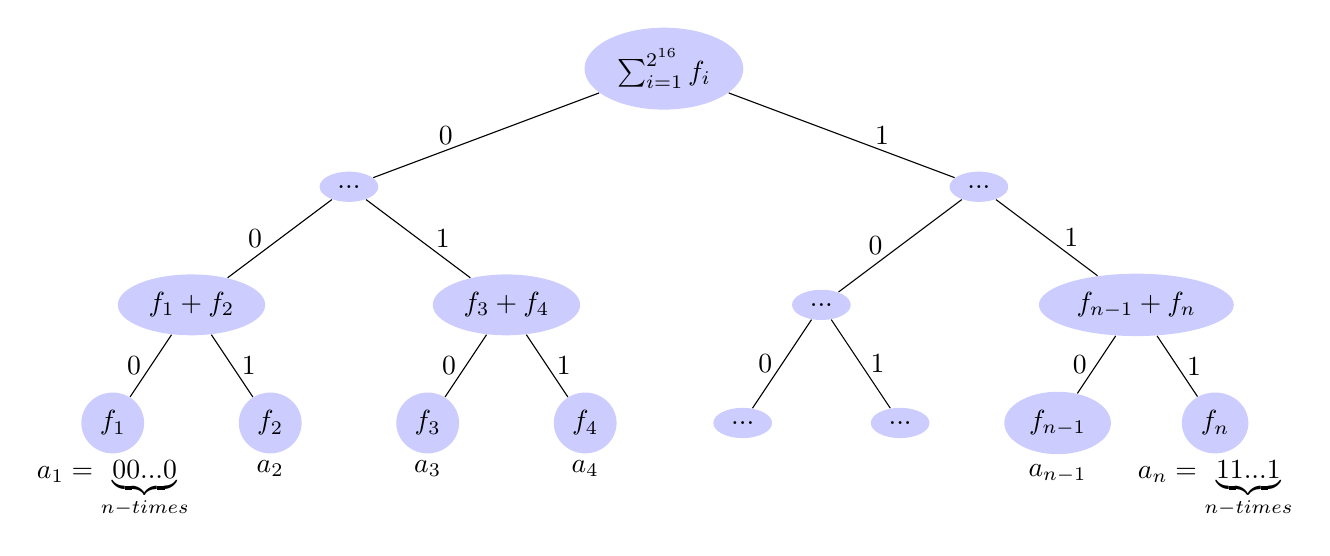
\begin{tikzpicture}[level distance=1.5cm,
            level 1/.style={sibling distance=8cm},
            level 2/.style={sibling distance=4cm},
            level 3/.style={sibling distance=2cm},
            tree node/.style={ellipse, fill = blue!20},
            every child node/.style={tree node}]
            
            \node[tree node] (Root) {$\sum_{i=1}^{2^{16}} f_i$}
                child {
                node {...} 
                child { node {$f_1+f_2$} 
                            child{ node (a1) {$f_1$} edge from parent node[left] {0}
                            }
                            child{ node (a2) {$f_2$} edge from parent node[right] {1}
                            }
                            edge from parent node[left  =0.1 cm] {0} }
                child { node {$f_3+f_4$} 
                            child{ node (a3) {$f_3$} edge from parent node[left] {0}
                            }
                            child{ node (a4) {$f_4$} edge from parent node[right] {1}
                            }
                            edge from parent node[right = 0.1 cm] {1} }
                edge from parent node[left = 0.3cm] {0} 
            }
            child {
                node {...}
                child { node  {...}  
                            child{ node (a5) {...} edge from parent node[left] {0}
                            }
                            child{ node (a6) {...} edge from parent node[right] {1}
                            }
                            edge from parent node[left = 0.1 cm] {0} }
                child { node  {$f_{n-1}+f_n$} 
                            child{ node (a7) {$f_{n-1}$} edge from parent node[left] {0}
                            }
                            child{ node (a8) {$f_n$} edge from parent node[right] {1}
                            }
                            edge from parent node[right = 0.1 cm] {1} }
                edge from parent node[right = 0.3 cm] {1}
            };
            \draw (a1) node[below = 0.35 cm,draw=none,fill=none](){$a_1=\underbrace{00...0}_{n-times}$};
            \draw (a2) node[below = 0.35 cm,draw=none,fill=none](){$a_2$};
            \draw (a3) node[below = 0.35 cm,draw=none,fill=none](){$a_3$};
            \draw (a4) node[below = 0.35 cm,draw=none,fill=none](){$a_4$};
            \draw (a7) node[below = 0.4 cm,draw=none,fill=none](){$a_{n-1}$};
            \draw (a8) node[below = 0.35 cm,draw=none,fill=none](){$a_n=\underbrace{11...1}_{n-times}$};
    
        \end{tikzpicture}
        \caption*{\textbf{Huffman encoding graph for 16-bit characters}, $n = 2^{16}$}
    
    \end{center}
    \end{figure}
\newpage
\section{Graduation Party of Alice}

\subsection{}
The following problem can be represented as a graph. With the $n$ people as the nodes of the graph and there is an edge between 2 nodes if the two people know each other. Once the graph is ready, we can make an adjacency list for the same in $O(m)$ time. $n->$ no. of people that are invited to the party and $m->$ no. of pairs who know each other (hence the number of edges in the graph will be $m$). We can maintain an array which will store the degree of each vertex and this can be done in $O(n+m)$ time using the adjacency list we have created above. Degree here will denote the number of people a person knows.
\\\\
\textbf{Claim 1:} Any node in the graph which has a degree less than 5 cannot be invited to the party.\\
\textbf{Proof of Claim 1:} Let $v_0$ be the vertex with degree less than 5. Now since this node has a degree less than 5, it means that he knows less than 5 people out of all the people who can be possibly invited to the party. Their is no such way by which he can know more people and hence the only option that is left with us is to remove him from the list of possible people who can be invited the party.
\\\\
Now we will keep removing the nodes of the graph which have a degree of less than 5. Notice that as we remove a vertex the degree of it's neighboring vertices will also change and we will have to update their degrees. Removing a node can cause reduction in degree of other nodes. If degree of those vertices fall below 5 then we can't invite them to the party either. We will have to remove them as well. Now this process will continue until every vertex in the graph has degree of at-least 5.
\\\\
Let the current number of nodes in the graph be $n'$. Now consider a node whose degree is more than $n'-6$. Then that person doesn't know less than 5 people and we must do something in this case. 
\\\\
\textbf{Claim 2:} Let $V$ be the current set of nodes and $n'$ be the size of $V$ (i.e. $n'= |V|$). Any vertex whose degree is more than $n'-6$ cannot be the part of our final optimal solution.\\
\textbf{Proof of Claim 2:} We will show that their is no final optimal solution in which it doesn't know less than 5 people of all the invited people. Consider the current state of node set $V$. We know that the final set which will be invited to the party will be a subset of the current $V$. Let the node with degree more than $n'-6$ be $v_0$. Now if any vertex is removed from $V$ (which is not $v_0$) then there are 2 possible cases. Either it is a neighbour of $v_0$, that is it knows $v_0$, or it is not a neighbour of $v_0$, it doesn't know $v_0$. If it doesn't know $v_0$ then removing it from $V$ only reduces the no. of people $v_0$ doesn't know. If we remove any node which is the neighbor of $v_0$, then removing them doesn't change the number of people $v_0$ doesn't know. Hence the only possibility is we have to remove $v_0$.
\\\\
Thus any vertex with degree more than $n'-6$ cannot be the part of our final solution and it must be removed from $V$. Removing that person might decrease the degree of other vertices as well. From Claim 1 and Claim 2 we know that all the vertices with degree less than 5 must be removed and all the vertices with degree more than $n'-6$ should also be removed and this process must continue until all the nodes left in the final $V$ has a degree atleast 5 and atmost $n'-6$. 
\\\\
Once such a $V$ is achieved then we can show that all of these people in $V$ can be invited to the party. Consider any node from the set $V$, let it be $v_1$. Now $v_1$ has a degree of more than 4 and thus it has atleast 5 neighbors and thus knows atleast 5 people who will come to the party (because inviting all of the people present in graph). Also it's degree is atmost $n'-6$ which means there are atleast 5 vertices that are not connected to $v_1$. Hence there are atleast 5 people whom $v_1$ doesn't know.\\Hence all of them can be invited to the party.
\\\\
The problem can be solved in $O(n+m)$ time, $m$ is the number of edges and $n$ is the number of nodes. The Pseudo code for it is written below. We can initially insert all the nodes in a Queue. Whenever any node is found to have a degree of less than 5 or more than n'-6, then it is removed and marked removed. All the nodes whose degrees are affected due to its removal are inserted again into the queue and their degrees are updated in the "degrees" array. This process continues until the queue is empty.
\\\\
\textbf{Algorithm:}
\lstinputlisting[firstline =3]{3a.txt}

\textbf{Proof of Correctness:}
\\
Initially, all the nodes are inserted in the queue "q" (lines 16-18). This ensures that all the nodes are analysed (checked that their degrees are in the required range) atleast once. We start traversing the queue from front and keep greedily removing nodes with current degree less than 5 or greater than n'-6 (lines 34-43). This step is justified by claim 1 and claim 2 given above. Now, whenever a node is removed, the degree of its current neighbours decreases and hence they are inserted again in the queue so that they are analysed atleast once more with updated degree before the queue becomes empty (lines 41-43). Thus, after the queue becomes empty, all the nodes that have not been marked as removed have degrees atleast 5 and less than n'-6 (n' is current number of nodes that are not removed). Thus, the algorithm returns the largest subset satisfying the given criteria.
\\\\
\textbf{Time complexity Analysis:}
\begin{enumerate}
    \item Making adjacency list takes $O(m)$, since we doing only $m$ iterations.
    \item Pushing degrees of vertices into Queue takes $O(n)$ time.
    \item Every removed node's adjacency list is traversed (atmost 1 time) and vertices with updated degree are inserted into Queue. This means maximum possible size of queue at any time could be $2*m$. Also, the number of times a particular node can be inserted in the Queue is equal to Degree+1 (since we are traversing adjacency list of only the nodes which will be marked as removed and any node is marked as removed atmost once). Since we are iterating in the while loop until the queue is empty, we do a maximum of $2*m$ iterations and in each we use front() function of queue whose complexity is $O(1)$. Thus the overall time taken is $O(m)$.
    \item Traversing the adjacency list takes $O(m)$ time and in each of that we put the updated degree. Adding element in Queue takes $O(1)$ time. Hence the total time taken by the Algorithm from line 37 to 43 over all the iterations of while loop is $O(m)$
\end{enumerate}
\textbf{Hence overall time-complexity is \boldmath{$O(n+m)$}}
\newpage
\subsection{}

Consider all of them are standing in a sorted order of their ages. Let us call them $a_1, a_2, a_3, a_4, ... , a_{n0}$. Thus we know that $age[a_1] <= age[a_2] <= age[a_3] ... <= age[a_{n0}]$. Now consider the table on which $a_1$ is sitting and let this table be $T$.
\\\\
\textbf{Claim 1:} If $a_k$ is sitting on $T$ (the table on which $a_1$ is sitting) in optimal arrangement and there exists a person (say $a_i$) with age less than $a_k$ not sitting on $T$ ( say he is sitting on table $T_1$), then there also exists an optimal solution in which $a_k$ is sitting in table $T_1$ and $a_i$ is sitting on table $T$.\\
\textbf{Proof of claim 1:} Let's say the person with age less than that of $a_k$ is $a_i$, $a_k$ is a person sitting on the table $T$ and $a_i$ is not sitting on the table $a_k$. Let's say $a_i$ was on the table $T_1$. We can exchange the position of $a_i$ and $a_k$ in this case. Because: (1) $a_i$ can be placed on table of $a_1$ in place of $a_k$ since $age[a_i] - age[a_1] <= age[a_k] - age[a_1]$. (2) The least age of a member on $T_1$ is greater than or equal to $age[a_1]$ and the max possible age of a person on $T_1$ can be $age[a_i]+10$ (since $a_i$ was on $T_1$). Since $a_k$ was sitting on $T$ so $age[a_k] - age[a_1]<= 10$. Also, $age[a_i] < age[a_k]$ (according to the assumption in the claim) which implies $(age[a_i]+10)-age[a_k] < 10$. Thus, we can also place $a_k$ in place of $a_i$ on T1. 
\\Thus, we can exchange $a_i$ and $a_k$. Keeping $a_k$ on the other table can provide more flexibility in age constraint on the other table.
\\\\
Now using the above we can place $S= {a_1, a_2, a_3 ... , a_m}$ people on the first table, here $m <=10$ and $age[a_m] - age[a_1] <=10$. Also $age[a_1] <= age[a_2] <= age[a_3] ... <= age[a_m]$. If $m< 10$ then either we don't have enough number of people or $age[m+1] - age[a1] >10$. 
\\
Let J be the set of all the people and S be the set that we have placed. Now define $J^* = J\backslash S$.
\\\\
\textbf{Claim 2:} $opt(J) = opt(J*) +1$, $opt(J)$ is the minimum number seats required to arrange the set of people $J$ on tables under the required constraints.\\
\textbf{Proof of Claim 2:}\\
We will show that both the below inequalities are true

$opt(J) <= opt(J^*) +1\hspace{1.5 cm}...(i)$

$opt(J)-1 >= opt(J^*)\hspace{1.5 cm}...(ii)$\\
Proof of (i):\\
After placing $S$ on 1 table we are left with $J\backslash S$ people and $opt(J^*)$ will place all of them on some table. And hence there exists one arrangement in which the arrangement can be done in $opt(J^*)+1$ no. of tables. Thus $opt(J) <= opt(J^*)+1$\\
Proof of (ii):\\
Let $A$ be the optimal arrangement of $J$ in which all the people in set $S$ are placed on a single table (say table $T$). Only they can be seated on that table. Now none of the people from $J\backslash S$ can be seated on table $T$ since either $T$ is full or their age is more than $age[a_1]+10$. Thus the $A\backslash T$ can be used to place all of the members of $J\backslash S$ i.e., $J^*$. Thus $J\backslash S$ members can be placed using $opt(J)-1$ tables. Hence one solution of size $opt(J)-1$ exists for $J^*$. This shows that $opt(J^*) <= opt(J)-1$.
\\\\
Hence from both $(i)$ and $(ii)$ we have, $opt(J)= opt(J^*)+1$.
\\\\
Now for calculating we can maintain a $freq$ array. $freq[i]$ denotes the number of people with age $i+10$. Now we can start placing them on tables in increasing order of age as we have discussed above, by recursively dividing the problem into a smaller sub-problem.
\\\\
\newpage
\textbf{Algorithm:}
\lstinputlisting[firstline =3]{3b.txt}
\textbf{Time complexity Analysis:}
\begin{enumerate}
    \item Making the $freq$ array needs $O(n_0)$ time.
    \item $j$ takes values till 90 only over all the iterations but it might be possible it is stuck at same position for some iterations.
    \item At a particular value of $j$, the inner while loop runs for $\lceil{freq[j]/10}\rceil$ times.
    \item Since the $freq[j]$ decreases by 10 in one iteration and sum of frequencies over all $j$ is $n_0$, hence the maximum possible number of times these loops can run is O($n_0/10$).
\end{enumerate}
\textbf{Thus the overall Time Complexity is \boldmath{$O(n_0)$}}


\end{document}
